%%%%%%%%%%%%%%%%%%%%%%%%%%%%%%%%%%%%%%%%%%%%%%%%%%%%%%%%%%%%%%%%%%%%%%%%
%                                                                      %
% LaTeX, FIIW thesis template                                          %
% 28/11/2014 v1.2                                                      %
%                                                                      %
%%%%%%%%%%%%%%%%%%%%%%%%%%%%%%%%%%%%%%%%%%%%%%%%%%%%%%%%%%%%%%%%%%%%%%%%
\documentclass[11pt,a4paper]{report}
% Indien je je thesis recto-verso wil afdrukken gebruik je onderstaande opties i.p.v. bovenstaande
%\documentclass[11pt,a4paper,twoside,openright]{report}

\usepackage[a4paper,left=3.5cm, right=2.5cm, top=3.5cm, bottom=3.5cm]{geometry}
\usepackage[dutch]{babel}
\usepackage{graphicx}
%\usepackage[latin1]{inputenc}           % om niet ascii karakters rechtstreeks te kunnen inputten
\usepackage[utf8]{inputenc}            % commentarieer deze regel uit als je utf8 encoded files gebruikt in plaats van latin1
\usepackage{natbib}
\usepackage{listings}             		% voor het weergeven van broncode
\usepackage{verbatim}					% weergeven van code, commando's, ...
\usepackage{hyperref}					% maak PDF van de thesis navigeerbaar
\usepackage{url}						% URL's invoegen in tekst met behulp van \url{http://}
\usepackage[small,bf,hang]{caption}     % om de captions wat te verbeteren
\usepackage[final]{pdfpages}            % gebruikt voor het invoegen van het artikel in pdf-formaat
\usepackage{pslatex}					% andere lettertype's dan de standaard types

\usepackage{sectsty}					% aanpassen van de fonts van sections en chapters
\allsectionsfont{\sffamily}
\chapterfont{\raggedleft\sffamily}

\usepackage{float}                      % De optie H voor de plaatsing van figuren op de plaats waar je ze invoegt. bvb. \begin{figure}[H]
%\usepackage{longtable}					% tabellen die over meerdere pagina's gespreid worden
%\usepackage[times]{quotchap}           % indien je fancy hoofdstuktitels wil
%\usepackage[none]{hyphenat}
%\usepackage{latexsym}
%\usepackage{amsmath}
%\usepackage{amssymb}

\usepackage{fiiw_gent}
% \usepackage{fiiw_ghent_eng} % For the english version (also change last page at the bottom of this file!

%door onderstaande regels in commentaar te zetten, of op false, kan je pagina's weglaten
%bijvoorbeeld het weglaten van een voorwoord, lijst met symbolen, ...
%%%%%%%%%%%%%%%%%%%%%%%%%%%%%%%%%%%%%%%%%%%%%%%%%%%%%%%%%%%%%%%%%%%%%%%%%%%%%%%%%%%%%%%%
%voorwoord toevoegen?
\acknowledgementspagetrue
\acknowledgements{voorwoord}			%.tex file met daarin het voorwoord
%abstract toevoegen?
\abstractpagetrue
\abstracts{abstract}					%.tex file met daarin het abstract
%lijst van figuren toevoegen?
\listoffigurespagetrue
%lijst van tabellen toevoegen?
\listoftablespagefalse
%lijst van symbolen toevoegen?
%\listofsymbolspagetrue
%\listofsymbols{symbolen}				%.tex file met daarin de lijst van symbolen



%informatie over het eindwerk, de promotor, ...
%%%%%%%%%%%%%%%%%%%%%%%%%%%%%%%%%%%%%%%%%%%%%%%
\opleiding{master of Science in de industri\"ele wetenschappen ICT}
\afdeling{Advanced Communicatie Technologies}

\title{Titel masterproef}
\subtitle{Ondertitel (facultatief)}
% \author{naam student}
\forename{Pieter-Jan}
\surname{Robrecht}
\academicyear{2016 - 2017}

\promotorA[Promotor(en)]{Annemie Vorstermans}
\promotorB[Co-promotor(en)]{Wim Vancroonenburg\\Carl Eeckhout}

\begin{document}
\selectlanguage{dutch}
% \selectlanguage{english} % For the english version
\preface

%Het eerste hoofdstuk van je thesis.
\chapter{Inleiding}
In dit hoofdstuk\index{hoofdstuk} gaan we een voorbeeld geven van een voetnoot\footnote{Dit is dus een voetnoot}. Een referentie naar hoofdstuk ~\ref{verwijzing}, dat zich op pagina \pageref{verwijzing} bevindt, is dus ook een koud kunstje. Zorg er wel voor dat je de namen van de labels een beetje verstandig kiest. Hoofdstukken label je het best als hfdstk:naam, plaatjes als img:naam en tabellen\index{tabellen} als tabel:naam. Zo verlies je zelf de bomen in het bos niet.
\newpage
SDffjfhd fsffh hsf
fh fhf
shf klfh
ffffsdfklfhklfhklfhhfklfhkldhffhsdfhfhfhfhfh
\newpage
dhfhffh hf fh fh fhfh fhfh hfh fhffhsdfhfhfhfhfhfhsdfh hfh fh
 




%second chapter of your thesis
\chapter{Bespreking}
In het vorig hoofdstuk hebben we naar deze tekst verwezen\label{verwijzing}.

%Hier worden de ontwikkelen van het prototype besproken.
%Achteraf komt er ook een conclusie van wat er allemaal goed was en wat er precies moet worden aangepast.
\chapter{Prototype}

\section{Uitwerking}

\section{Testen}

You can say great work has been done about something \citep{Castleman98,Granlund95} or say that \citet{Holmes95} did something really great.
%In dit hoofdstuk zal worden herhaald wat er moet worden aangepast afhankelijk van de uitkomst van het prototype.
%Er zal gekeken worden naar alternatieve werkwijzes of eventuele uitbreidingen van het prototype.
%De resultaten van de testen worden hier ook besproken.
\chapter{Eind product}

\section{Uitwerking}

\section{Testen}
%Hier komt dan de conclusie en terug koppeling
\chapter{Conclusie}

% Bibliografie: referenties. De items zitten in bibliografie.bib
%%%%%%%%%%%%%%%%%%%%%%%%%%%%%%%%%%%%%%%%%%%%%%%%%%%%%%%%%%%%%%%%%
% Indien je ook de niet geciteerde werken in je bibliografie wil opnemen, commentarieer dan onderstaande regel uit!
%\nocite{*}
\bibliographystyle{apalike}
\bibliography{bibliografie}

% Eventueel enkele appendices
%%%%%%%%%%%%%%%%%%%%%%%%%%%%%%
\appendix
\chapter{Een aanhangsel}
sdfsffqsfsf

% Bijlage met daarin het wetenschappelijk artikel
%%%%%%%%%%%%%%%%%%%%%%%%%%%%%%%%%%%%%%%%%%%%%%%%%%
\chapter{Beschrijving van deze masterproef in de vorm van een wetenschappelijk artikel}
%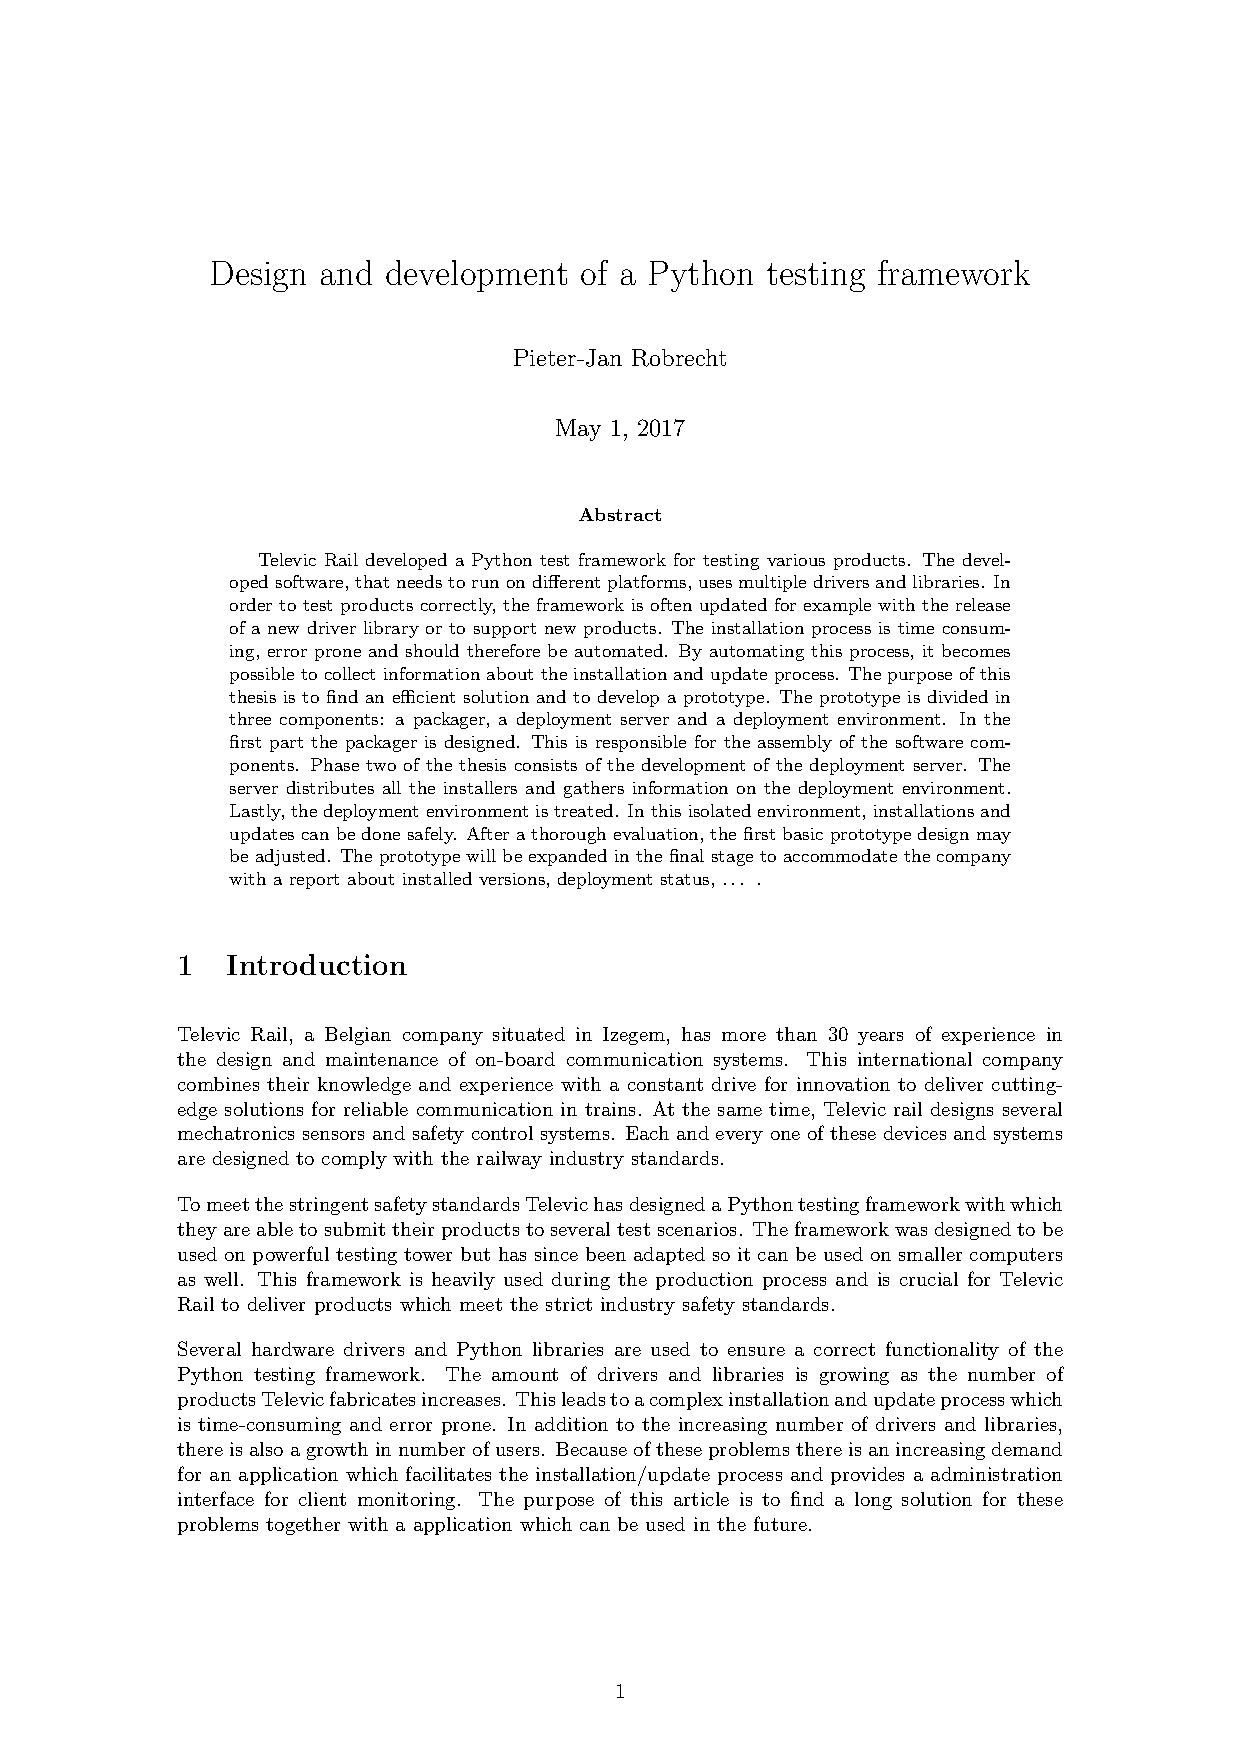
\includepdf{artikel.pdf}

% Bijlage met daarin de poster
%%%%%%%%%%%%%%%%%%%%%%%%%%%%%%%
\chapter{Poster}
%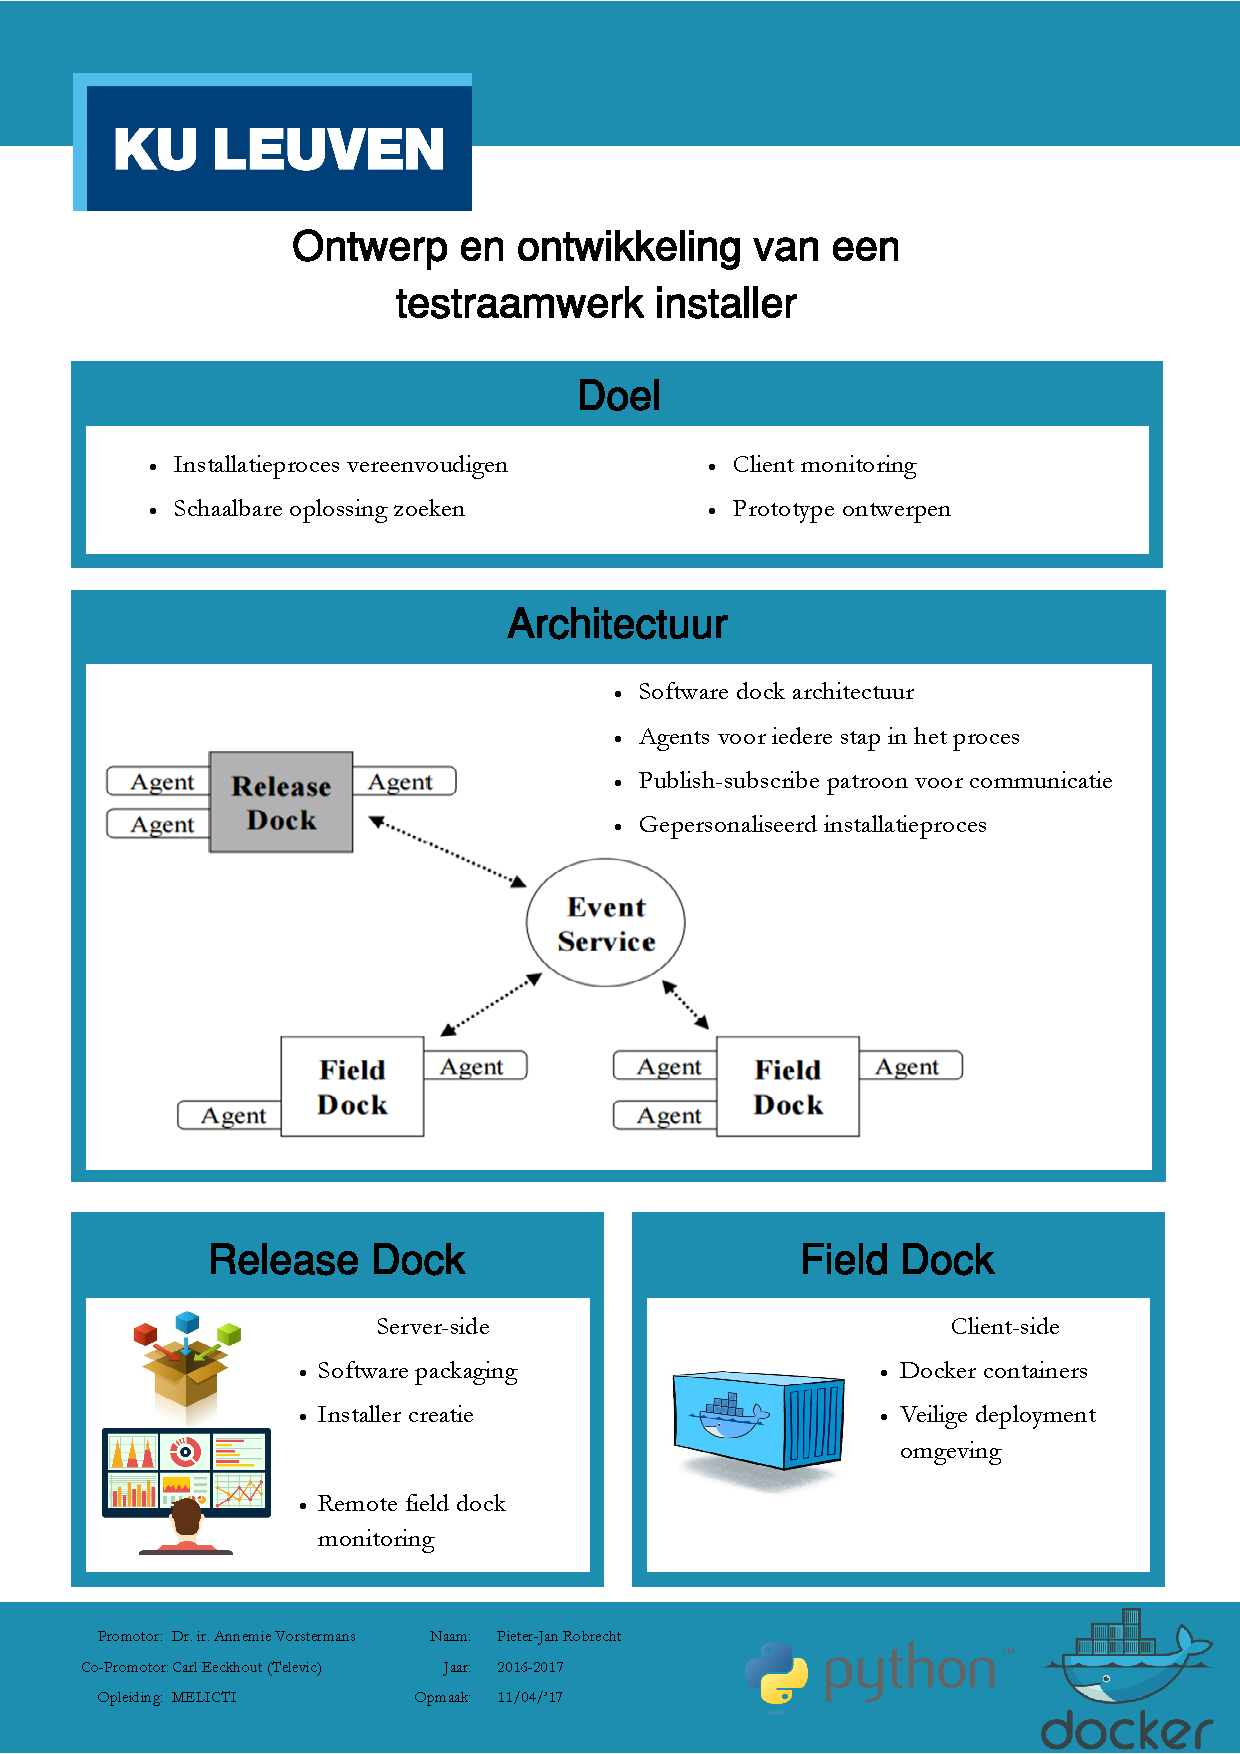
\includepdf{poster.pdf}


\includepdf{back_fiiw_gent.pdf}
% 
\includepdf{back_fiiw_ghent_eng.pdf} % For the english version

\end{document}
